
\section[Files and Chunks]{A (very quick) overview of data in swarm}



\subsection{Data in}
% \wholeslide{Data in: Saving data to the swarm.}
\blockslide{\textbf{Data in}}{Saving data to the swarm.}
\subsubsection{Chunking}
\wholeslide{1. Chunking: breaking up the data}

\begin{frame}[t]{\alt<5->{It's chunks all the way down...}{Chunks}}
% \begin{overlayarea}{⟨area width⟩}{⟨area height⟩}
%   ⟨environment contents⟩
% \end{overlayarea}
\begin{overlayarea}{\textwidth}{10cm}
Under the hood swarm does not deal in files but in \emph{chunks.}

\begin{itemize}
 \item<2-> All data is broken into pieces of size 4kB: ``chunks".
 \item<4-> Chunks are hashed and the hash is used as their ID/address.
 \item<5-> Chunk hashes are also packaged into 4kB chunks...
\end{itemize}

\begin{onlyenv}<1-2>
 \begin{center}
  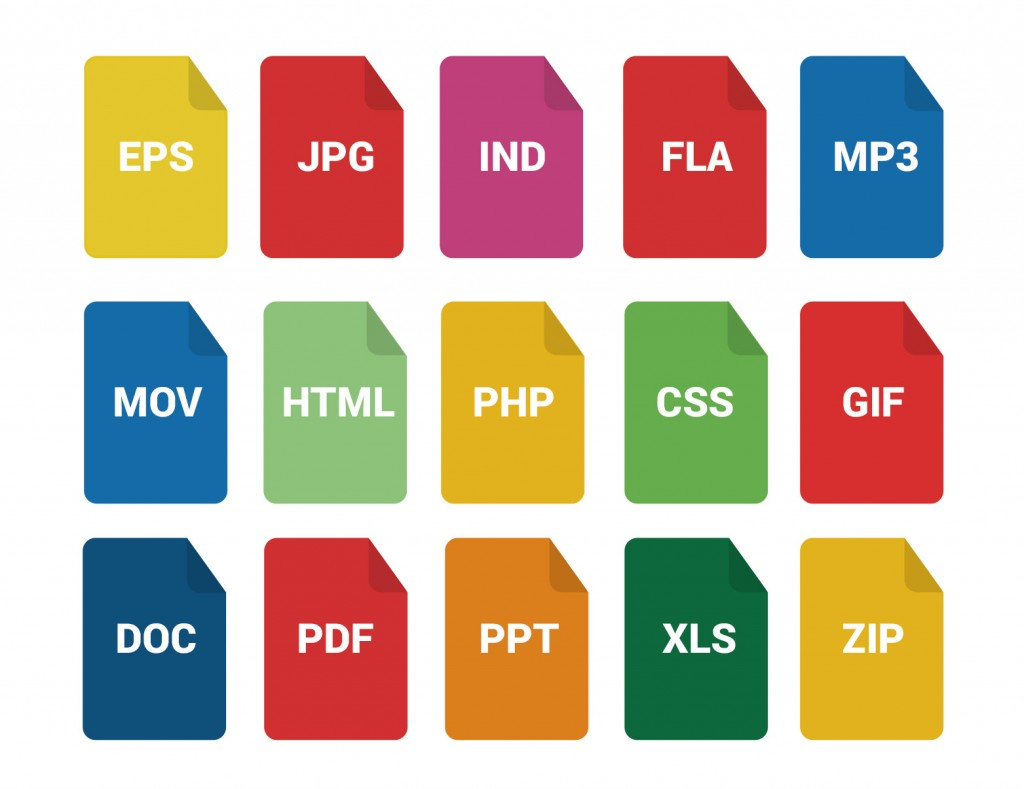
\includegraphics[width=0.4\textwidth]{files.jpg}
  \transdissolve<3>
 \end{center}
\end{onlyenv}

 \begin{center}
  \begin{tikzpicture}
   \node[chunk,visible on=<3>] at (0,0) (achunk){};
   \node[visible on=<3>] at (-1.8,0) (labeltext){A ``chunk:"};
   \node[chunk,visible on=<3->] at (-4,-3) (a){};
   \node[chunk,visible on=<3->] at (-2,-3) (b){};
   \node[chunk,visible on=<3->] at (0,-3) (c){};
   \node[chunk,visible on=<3->] at (2,-3) (d){};
   \node[chunk,visible on=<3->] at (4,-3) (e){};

   \node at (-4.2,-1.3) (dummy1) {};
   \node at (4.2,-1.7) (dummy2) {};
   \node[chunk,fit=(dummy1)(dummy2),visible on=<5>]{};

   \node[scale=0.8,draw,visible on=<4-5>] at (-4,-1.5) (ha){$h_1$}
     (a.north) edge[-,visible on=<4>] (ha.south);
   \node[scale=0.8,draw,visible on=<4-5>] at (-2,-1.5) (hb){$h_2$}
     (b.north) edge[-,visible on=<4>] (hb.south);
   \node[scale=0.8,draw,visible on=<4-5>] at (0,-1.5) (hc){$h_3$}
     (c.north) edge[-,visible on=<4>] (hc.south);
   \node[scale=0.8,draw,visible on=<4-5>] at (2,-1.5) (hd){$h_4$}
     (d.north) edge[-,visible on=<4>] (hd.south);
   \node[scale=0.8,draw,visible on=<4-5>] at (4,-1.5) (he){$h_5$}
     (e.north) edge[-,visible on=<4>] (he.south);

   \node[chunk,visible on=<6>] at (0,-1.5) {};
     \end{tikzpicture}

 \end{center}
\end{overlayarea}
\end{frame}

\subsubsection{Encoding}
\wholeslide{2. Encoding: Assembling the chunks into a merkle tree.}

\begin{frame}[t]{Everything is merkle-ised.}
When you want to save a document (or collection) to swarm, the swarm client
\begin{enumerate}
 \item<2-> Assembles all chunks into a merkle tree...
 \item<3-> ...including extra redundancy (``parity chunks").
 \item<4-> Returns a single \textbf{root hash} for the entire collection.
\end{enumerate}
\uncover<5->{\textbf{Note:} This means that you entire collection is accessible and retrievable from this single hash.}

\begin{center}
 \begin{onlyenv}<2>
  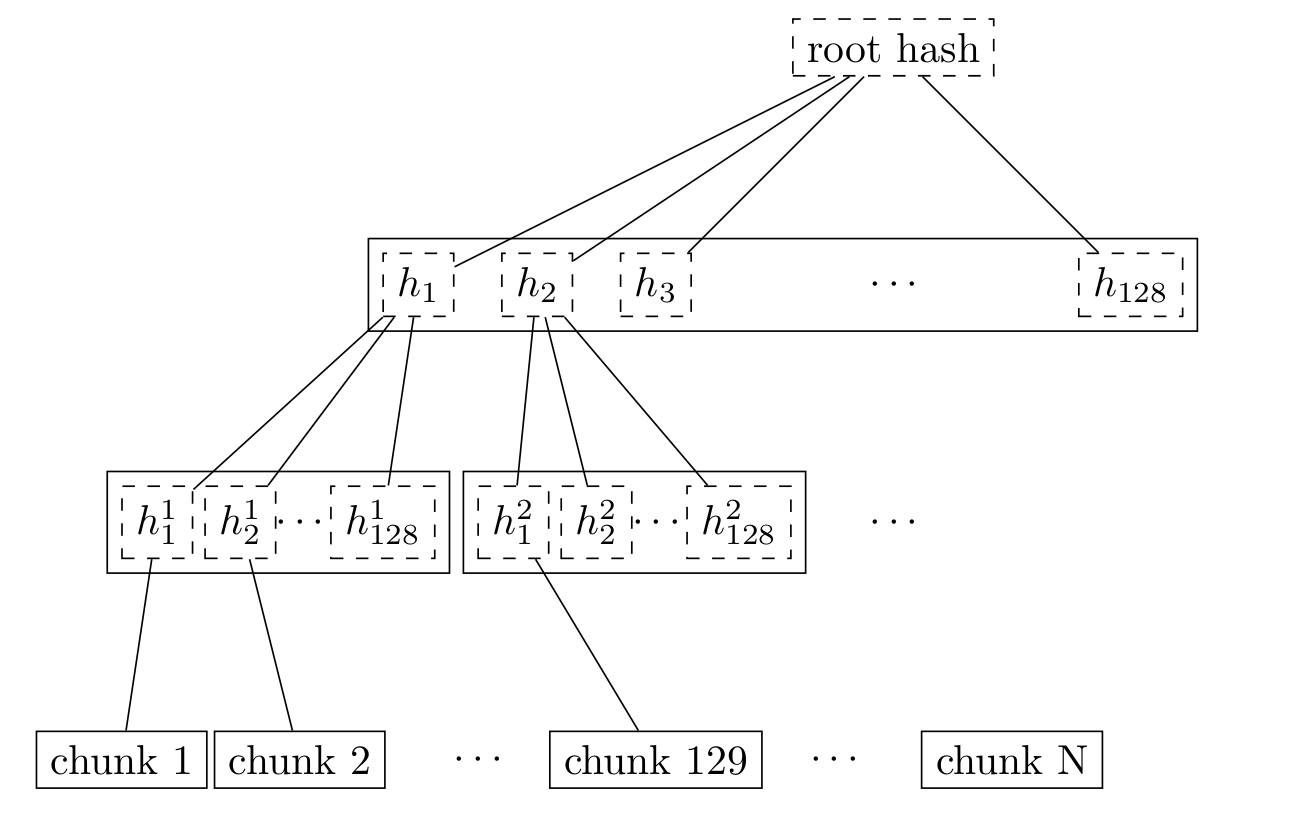
\includegraphics[width=0.5\textwidth]{chunk-tree.png}
 \end{onlyenv}
 \begin{onlyenv}<3>
  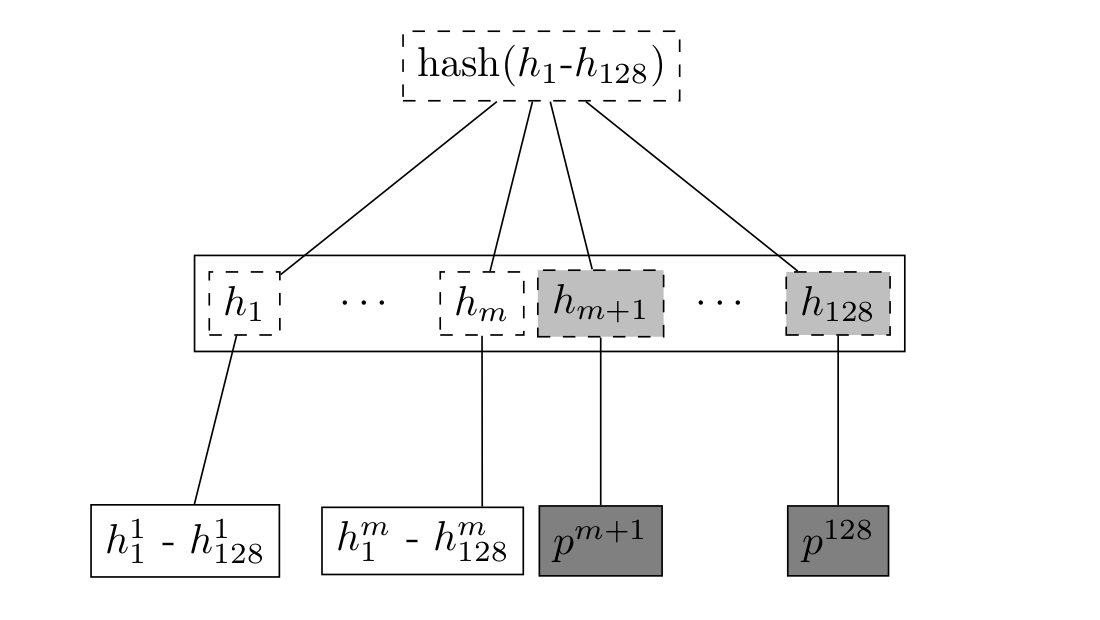
\includegraphics[width=0.5\textwidth]{erasure-coded-tree.png}
 \end{onlyenv}

\end{center}



\end{frame}



\subsubsection{Syncing}
\wholeslide{3. Syncing: getting the chunks to where they need to be.}

\begin{frame}{The syncing process.}
\begin{columns}[T]
\begin{column}{0.4\textwidth}
\small{The process of getting chunks to their storage destination is called \alert<1>{syncing}.}

\begin{itemize}
 \item<3-> \alt<5->{\tiny}{} Chunks are to be stored at\alt<4->{\alert<4>{ the node whose address is closest to}}{} the chunk ID.
 \item<5-> \alt<7->{\tiny}{} Instead of directly connecting to that node and giving it the chunk in question, we pass the chunk along to one of our connected peers who is a little closer to the chunk ID than we are. \uncover<6->{``Syncing".}
 \item<7-> \alt<10->{\tiny}{} This peer will repeat the process, thus the data is passed on \uncover<8->{from node}\uncover<9->{ to node.}
 \item<10>[] %dummy. I needed this to get line spacing to work in the point above.
\end{itemize}
{  }\pause
\end{column}

\begin{column}{0.6\textwidth}
\begin{tikzpicture}
 \node[scale=0.7]{
    \begin{tikzpicture}
	\node[invisible] at (0,-9) (dummy){};
	\node[invisible] at (5,-5) (dummy2){};
	\node[peer,visible on=<2->] at (-2,0) (owner){Owner};

	\node[visible on=<3->] (chunk) at (4,-5) {$\bullet$};
	\node[visible on=<3->] (chunklabel) at (5,-4) {chunk address} edge[point,->,visible on =<3->] (chunk);

	\node[peer,visible on=<5->] at (0.5,-0.5) (connectedpeer){peer}
	    (owner.east) edge[point, ->,visible on=<6->, bend left=15]
		    node[above=2pt,visible on=<6->] {sync}
			    (connectedpeer.150);

	\node[node,visible on=<7->] at (1,-2) (firstnode){some node}
		(connectedpeer.-70) edge[point,->,visible on=<7->,bend left=10]
		    node[right of=2pt,visible on=<7->] {sync}
			    (firstnode.north);

	\node[node,visible on=<8->] at (0.5,-4.5) (secondnode){other node}
		(firstnode.-70) edge[point,->,dashed,visible on=<8->,bend left=10]
		    node[right of=2pt,visible on=<8->] {syncing...}
			    (secondnode.70);

	\node[peer,visible on=<4->] at (4,-6) (closestnode){closest node}
		(secondnode.-110) edge[point,->,visible on=<9->,out=-110,in=180]
		    node[above=2pt,visible on=<9->] {sync}
			    (closestnode.west);
    \end{tikzpicture}
    };
\end{tikzpicture}
\end{column}
\end{columns}

\end{frame}

\wholeslide{ }

\subsection{Data out}

% \wholeslide{Data out: How to retrieve data stored in the swarm.}
\blockslide{\textbf{Data out}}{How to retrieve data stored in the swarm.}

\begin{frame}{Data Retrieval}
 When retrieving data from the swarm remember:
 \begin{itemize}
  \item<2-> All data is in chunks.
  \item<3-> All chunks are addressed by their hashes.
  \item<4-> Chunks are stored on nodes that are closest to the chunk hash.
 \end{itemize}
\end{frame}

\begin{frame}

\begin{tikzpicture}
\node[peer,visible on=<1->] at (12,0) (retriever){Retriever};
\node[visible on=<13>,scale=2] at (12,-1) {\Smiley};

\node[visible on=<2->] (chunk) at (4,-5) {$\bullet$};
\node[visible on=<2->] (chunklabel) at (3,-4) {chunk address} edge[point,->,visible on =<2->] (chunk);

\node[peer,visible on=<4-12>, dimmed on=<13->] at (8.5,-0.5) (connectedpeer){peer}
    (retriever.-150) edge[point, ->,visible on=<5>,dimmed on=<6-12>,  bend left=15]
	    node[below=2pt,visible on=<5>, dimmed on=<6-12>] {request}
		    (connectedpeer.-10);

\node[node,visible on=<6-11>, dimmed on=<12->] at (6,-2) (firstnode){some node}
	(connectedpeer.-70) edge[point,->,visible on=<6>, dimmed on=<7-11>,bend left=30]
	    node[right of=2pt,visible on=<6>, dimmed on=<7-11>] {request}
		    (firstnode.east);

\node[node,visible on=<7-10>, dimmed on=<11->] at (7.5,-4.5) (secondnode){other node}
	(firstnode.-70) edge[point,->,dashed,visible on=<7>, dimmed on=<8-10>,bend left=10]
	    node[right of=2pt,visible on=<7>, dimmed on=<8-10>] {requests...}
		    (secondnode.120);

\node[peer,visible on=<3-9>, dimmed on=<10->] at (4,-6) (closestnode){closest node}
	(secondnode.-110) edge[point,->,visible on=<8>, dimmed on=<9>,out=-110,in=0]
	    node[right of=2pt,visible on=<8>, dimmed on=<9>] {request}
		    (closestnode.east)
	(closestnode) edge[thick,point,->,visible on=<9>] node[above=2pt,visible on=<9>]{deliver} (secondnode)
	(secondnode.north west) edge[thick, point,->,visible on=<10>, dashed] node[left of=2pt,visible on=<10>]{deliveries} (firstnode.-120)
	(firstnode.55) edge[thick,point,->,visible on=<11>] node[left of=2pt,visible on=<11>]{deliver} (connectedpeer.-150)
	(connectedpeer) edge[thick,point,->,visible on=<12>] node[above=2pt,visible on=<12>]{deliver} (retriever)
	;
\end{tikzpicture}
\end{frame}
